\begin{frame}{}
    \LARGE Advanced Diffusion Models: \textbf{Classifier-Free Guidance}
\end{frame}

\begin{frame}[allowframebreaks]{Classifier-Free Guidance}
    \textbf{What is Classifier-Free Guidance?}
    \begin{itemize}
        \item It's a trick used in image generation models (like diffusion models).
        \item Lets us control how much the model listens to our prompt (like a text description) without needing a separate classifier.
        \item Makes the model more flexible and easier to use.
    \end{itemize}

    \framebreak

    \begin{figure}
        \centering
        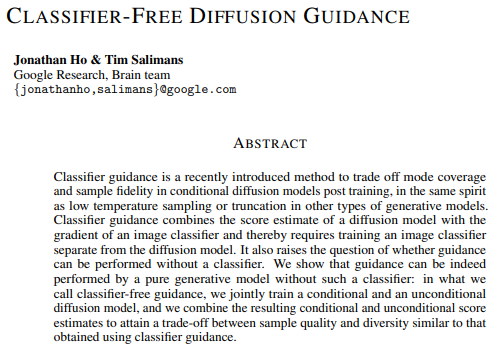
\includegraphics[width=0.8\linewidth,height=\textheight,keepaspectratio]{images/adv-img-gen/classifier-free-guidance-1.png}
        \caption*{[Ho et al., 2022](https://arxiv.org/abs/2207.12598)}
    \end{figure}

    \framebreak

    \textbf{How does it work?}
    \begin{itemize}
        \item The model is trained in two ways:
        \begin{itemize}
            \item \textbf{With prompt:} The model gets a text prompt and learns to generate images that match it.
            \item \textbf{Without prompt:} The model ignores the prompt and just generates images freely.
        \end{itemize}
        \item At generation time, we ask the model for both versions:
        \begin{itemize}
            \item One with the prompt (conditional).
            \item One without the prompt (unconditional).
        \end{itemize}
        \item We mix these two outputs to control how much the prompt matters.
    \end{itemize}

    \framebreak

    \textbf{The math (don't worry, it's simple!):}
    \[
        \epsilon_{\text{guided}} = \epsilon_\theta(\mathbf{x}_t, t, \mathbf{c}) + w \left[ \epsilon_\theta(\mathbf{x}_t, t, \mathbf{c}) - \epsilon_\theta(\mathbf{x}_t, t, \varnothing) \right]
    \]
    \begin{itemize}
        \item $\epsilon_\theta(\mathbf{x}_t, t, \mathbf{c})$: Output with the prompt.
        \item $\epsilon_\theta(\mathbf{x}_t, t, \varnothing)$: Output without the prompt.
        \item $w$: How strongly we want to follow the prompt.
    \end{itemize}

    \framebreak

    \textbf{What does $w$ do?}
    \begin{itemize}
        \item $w = 0$: Ignore the prompt (model is creative, less controlled).
        \item $w = 1$: Use the prompt as normal.
        \item $w > 1$: Really focus on the prompt (more faithful to what you asked).
    \end{itemize}

    \framebreak

    \begin{figure}
        \centering
        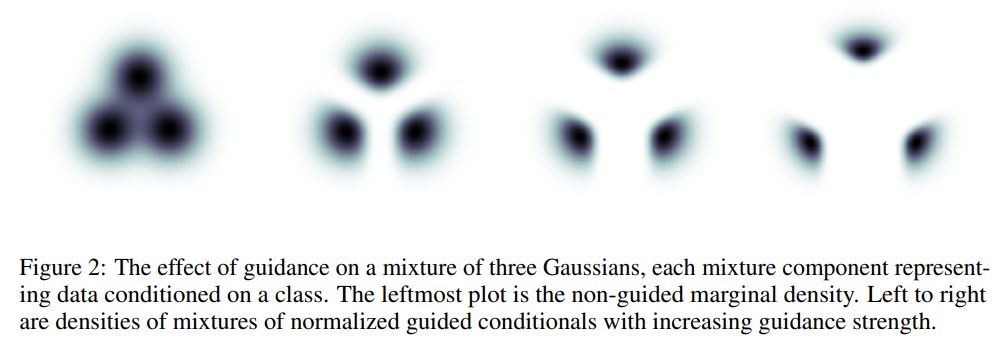
\includegraphics[width=\linewidth,height=\textheight,keepaspectratio]{images/adv-img-gen/classifier-free-guidance-2.png}
        \caption*{[Ho et al., 2022](https://arxiv.org/abs/2207.12598)}
    \end{figure}

    \framebreak

    \begin{figure}
        \centering
        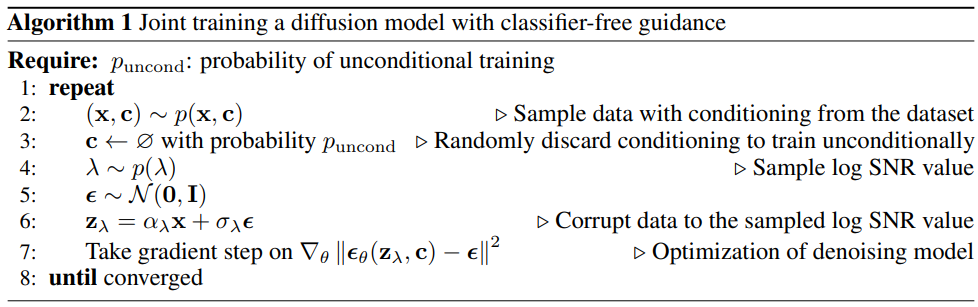
\includegraphics[width=\linewidth,height=\textheight,keepaspectratio]{images/adv-img-gen/classifier-free-guidance-3.png}
        \caption*{[Ho et al., 2022](https://arxiv.org/abs/2207.12598)}
    \end{figure}

    \framebreak

    \begin{figure}
        \centering
        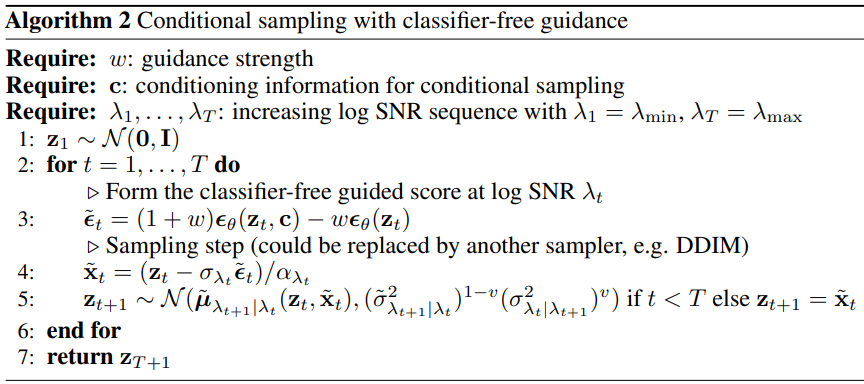
\includegraphics[width=\linewidth,height=\textheight,keepaspectratio]{images/adv-img-gen/classifier-free-guidance-4.png}
        \caption*{[Ho et al., 2022](https://arxiv.org/abs/2207.12598)}
    \end{figure}

    \framebreak

    \begin{figure}
        \centering
        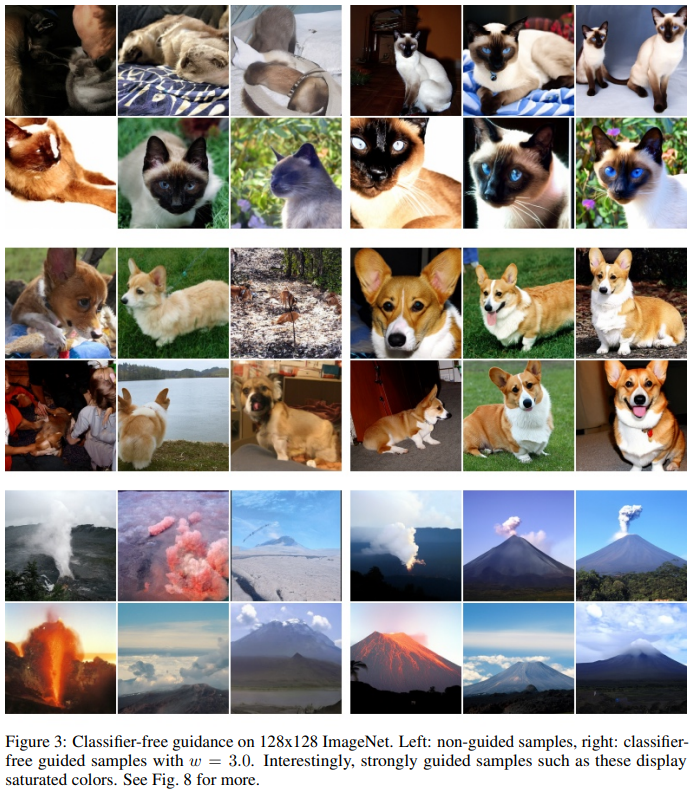
\includegraphics[width=\linewidth,height=0.9\textheight,keepaspectratio]{images/adv-img-gen/classifier-free-guidance-5.png}
        \caption*{[Ho et al., 2022](https://arxiv.org/abs/2207.12598)}
    \end{figure}

    \framebreak

    \begin{figure}
        \centering
        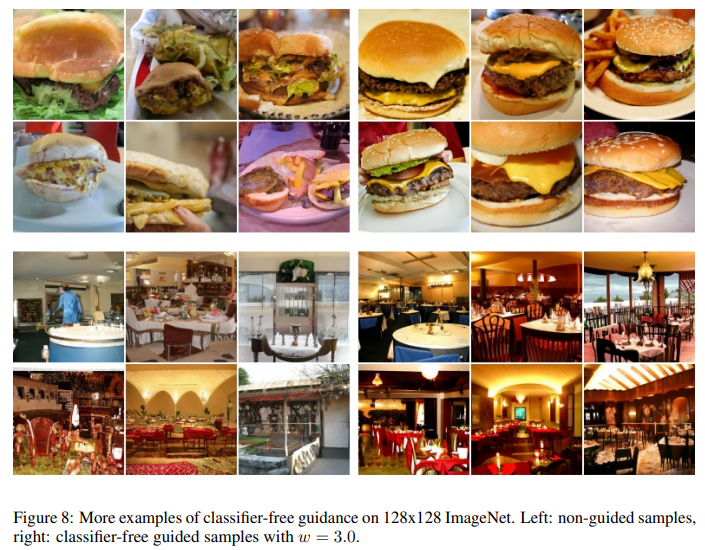
\includegraphics[width=\linewidth,height=0.85\textheight,keepaspectratio]{images/adv-img-gen/classifier-free-guidance-6.png}
        \caption*{[Ho et al., 2022](https://arxiv.org/abs/2207.12598)}
    \end{figure}
\end{frame}